%%%%%%%%%%%%%%%%%%%%%%%%%%%%%%%%%%%%%%%%%%%%%%%%%%%%%%%%%%%%%%%%%%%%%%%%%%%%%%%%
% setup.tex
% Main tex file for setup and content collocation
% For the use of University of Amsterdam
% Information Systems and Data Science students
% Adapted by Riccardo Fiorista (riccardo.fiorista@proton.me)
%%%%%%%%%%%%%%%%%%%%%%%%%%%%%%%%%%%%%%%%%%%%%%%%%%%%%%%%%%%%%%%%%%%%%%%%%%%%%%%%

% Options:
% Choose one of:
%% `is` - Information Systems
%% `ds` - Data Science 
% Add (separated by `,`):
%% `nolinenumbering` - If you want to remove line numbering on submission
%% `draftmargins` - If you would like to give your reviewer more space for comments
%% `nofrontpicture` - If you do not wish to have a graphic on your front-page
%% `nofirstcompanypicture` - If you do not wish to have a graphic on your front-page
%% `nosecondcompanypicture` - If you do not wish to have a graphic on your front-page
\documentclass[ds, nolinenumbering, nofrontpicture, nofirstcompanypicture, nosecondcompanypicture]{mscthesis}

%%%%%%%%%%%%%%%%%%%%%%%%%%%%%%%%%%%%%%%%%%%%%%%%%%%%%%%%%%%%%%%%%%%%%%%%%%%%%%%%
% DOCUMENT METADATA
%%%%%%%%%%%%%%%%%%%%%%%%%%%%%%%%%%%%%%%%%%%%%%%%%%%%%%%%%%%%%%%%%%%%%%%%%%%%%%%%

% Thesis related entries
\title{Gentrification in Storefront Signage in Amsterdam}
\subtitle{A Machine Learning Approach with Street View Imagery}

% Date on which your thesis is submitted
\date{Fill In The Date In Format DD.MM.YYYY}

% 4-5 keywords should do the trick. They should ideally be phrases of 2-4 words or single words.
% \keywords{gentrification, street view imagery, storefront signage, scene-text analysis, classification}

% Author data
\authorname{Anh Tran}
\authorid{12770698}
\authoremail{anh.tran1@student.uva.nl}

% Supervisors
\uvasupervisorname{Tim Alpherts}
\uvasupervisoraffiliation{UvA Supervisor}
\uvasupervisoremail{t.o.l.alpherts@uva.nl}

% Comment if you do not have an external supervisor
% \externalsupervisorname{External Supervisor}
% \externalsupervisoraffiliation{External Supervisor}
% \externalsupervisoremail{supervisor@company.nl}

% % Uncomment and fill paths if you want to add custom images
% %% Figure size suggestions (in general it's best to render them from SVGs):
% %% 3000x3000 @ 240dpi for all three
% \titlepicturepath{}
% \firstcompanypicturepath{}
% \secondcompanypicture{path}

%%%%%%%%%%%%%%%%%%%%%%%%%%%%%%%%%%%%%%%%%%%%%%%%%%%%%%%%%%%%%%%%%%%%%%%%%%%%%%%%
% CONTENT
%%%%%%%%%%%%%%%%%%%%%%%%%%%%%%%%%%%%%%%%%%%%%%%%%%%%%%%%%%%%%%%%%%%%%%%%%%%%%%%%

\begin{document}

\pagestyle{plain}
\setcounter{page}{1}

% \maketitlepage
\fixemptypage

% \begin{abstract}
% % A summary of results should be included. Avoid citations. Maximum length is 200 words.
% Write your abstract here.
% \end{abstract}

\maketitle

% \section*{Github Repository}
% \url{https://github.com/atran13/MSc-Thesis-Gentrification-and-storefront-signage}

% Sections; Try to stick to this setup but you can comment each section
% \section{Introduction}
\label{sec:introduction}
% Mention scientific context/field, problem statement, research gap and candidate (sub) research question(s). 

Within urban studies, gentrification is a phenomenon widely discussed. First coined by British sociologist Ruth Glass in 1964 in her work about the inner city of London \cite{Glass1964}, the term refers to a neighborhood changing as a result of wealthier residents moving in, gradually displacing existing residents as local housing and service prices increase, and cultures homogenized or replaced. Gentrification thus involves an economic and demographic shift, as well as changes in the aesthetics of the built environment. For its negative effects on marginalized communities, it is worthwhile to understand and detect gentrification. This study took a focus on the visual indicators of gentrification, as visual elements are arguably the most telling factor of a neighborhood’s cultural identity, demographic and economic characteristics.

Gentrification is a multi-dimensional and multi-step process. Döring and Ulbricht \cite{döring_ulbricht_2018} defined gentrification as having 4 aspects: functional (establishment of businesses and cultural institutions), architectural (upgrade to the built environment), social (marginalization, displacement and replacement of existing residents), and symbolic (communication of a new image of the neighborhood to the wider public). As has been noted by Feiereisen and Sassin \cite{feiereisen_sounding_2021}, the functional, architectural, and symbolic aspects can be seen as constituting the visual indicators of gentrification. While these aspects take shape in multiple characteristics of the built environment, storefront signage (hereafter: signage) is a rich communication medium that embodies all three aspects. It is through signage that businesses directly establish their presence, communicate their commercial purposes and values, and distinguish themselves via a curated aesthetics \cite{rahman_signage_2020}. Furthermore, businesses understand the socio-cultural values and identity of the neighborhood, and thus design their appearance to best attract and serve this audience:

\begin{displayquote}
    "Shop signs are public texts that communicate what stores sell, who is perceived to be on the street and what their commercial desires are thought to be. [...] Similar to spoken utterances and all written texts, signs are designed for particular audiences [...]. Well-crafted stories are place-making tools inasmuch as they maintain and reproduce prevailing cultural standards and values." \cite{trinch_signsays_2017}
\end{displayquote}

It can therefore be expected that once there is a change in the neighborhood - demographically and economically (i.e. gentrification) - signage would act as a mirror for this change. Analyzing signage can help understand gentrification, and this is where the interest of the current study lies.

Existing research into the visual indicators of gentrification often analyzes elements such as improvements in the neighborhood's physical appearance and changes in architecture style \cite{huang_detecting_2022, ravuri_gsv_2022, naik_computer_2017, ilic_deepmap_2019}. Comparisons have been drawn in terms of old versus new features, openness of the properties (e.g. boarded up windows, fences), greenery, colors,...; but not as much attention has been paid to signage as a standalone feature. Most research that has been done in this regards are in the context of the US, in which clear distinctions were noted between gentrified and non-gentrified storefront signage \cite{trinch_signsays_2017, snajdr_oldschool_2018, snajdr_preserve_2022, rahman_signage_2020}. The vast majority of these studies on signage employs qualitative methods, whereby the researchers conduct observational data collection (i.e. manually photographing facades) and summarize what is present in their samples. While their findings provide invaluable insights, their methodologies are undoubtedly labor intensive. Furthermore, as has been pointed out by Reades et al. \cite{reades_understanding_2019} and Barton \cite{barton_exploration_2016}, such selection of neighborhoods and facades per neighborhood often comes with limitations in terms of generalizability on a city-wide scale. Conclusions made were about the most typical and differentiating characteristics, but to which extent are these characteristics present in the neighborhood, and in the city? Can it really be assumed that all signage from a gentrified neighborhood look the same? If not - i.e. if there exist outlying cases of non-gentrified storefronts in a gentrified neighborhood - what can be said about the actual state of gentrification, for instance in terms of the neighborhood demographic makeup? These are some nuances that existing research has not discussed, presumably due to their selection of data and limiting methodologies.

On the other hand, the growing availability of street view data and machine learning techniques has led to developments in Urban Visual Intelligence \cite{zhanga_urban_2023}, whereby cities' built environments are understood in conjunction with socio-economic circumstances and residents' activities on a large scale. Besides predictive modelling for gentrification \cite{thackway_build_2021, reades_understanding_2019}, work has been done to visually measure gentrification via documenting changes \cite{ravuri_gsv_2022}, detect \cite{huang_detecting_2022} and deep-map gentrification to reveal areas becoming gentrified \cite{ilic_deepmap_2019}. A small number of machine learning research took a focus on signage, but in terms of linguistic landscape \cite{hong_linguistic_2020, thung_detecting_2022}, typeface (font type) \cite{ma_typef_2019}, or to classify points of interest \cite{noorian_detect_2020, bakaev_stsem_2019}, instead of to understand the aesthetics of signage. Systematic literature reviews on Urban Visual Intelligence \cite{biljecki_street_2021, zhanga_urban_2023} have noted its applicability and importance in generating insights and decision-making, while pointing future research to further analyze written languages in images, as well as between-place inference (applying a machine learning model trained with one area to another). This study positions itself in this research gap, where it aims to expand the knowledge of signage aesthetics as a mirror of gentrification in Amsterdam, while utilizing computer vision and street view imagery to overcome limitations of existing urban ethnographic studies.

The dataset at the center of this research is from the StreetSwipe project. Using crowdsourcing, StreetSwipe \cite{streetswipe} lets people decide whether facades in Amsterdam appear gentrified. With this data, the study drew conclusions based on the subjective and common perception of a diverse group of people - arguably a necessity when it comes to a multi-faceted phenomenon such as gentrification. Moreover, with the images taken from all over the city, the results were not constrained per neighborhoods. Understanding the visual state of gentrification would help detect potential areas undergoing gentrification. As a pilot case, the main goal of the study was to see to which extent a computer vision model can learn the visual perception and, correspondingly, classify signage as perceptually gentrified or non-gentrified. Subsequently, with added data from areas of the city that was not covered in StreetSwipe, the model was tested to quantify the extent to which the perception hold against the actual state of the neighborhoods (i.e. given all signage from a gentrified neighborhood (as per census data), how much of the signage would be visually perceived as gentrified?). Lastly, via inspecting the model's predictions, insights were provided into the characteristics of gentrified and non-gentrified signage in Amsterdam, as well as cases where the distinction was less clear.

The research question of this study was stated as follow: 

\noindent\textit{To which extent can a computer vision model learn the differences between perceptually gentrified and non-gentrified storefront signage? How do the learned characteristics generalize to other neighborhoods of the city? Lastly, what are the characteristics that distinguish between gentrified and non-gentrified signage, and which characteristics make the distinction less clear?}

\begin{enumerate}
    \item Sub-RQ 1: To which extent can the scene-text detection model CRAFT identify signage from street view images?
    \item Sub-RQ 2: To which extent can fine-tuned ResNets correctly classify gentrified and non-gentrified StreetSwipe signage?
    \item Sub-RQ 3: How does the model trained on visual perception (StreetSwipe) perform on a test set of data from other neighborhoods, labeled per census data (the extended dataset)?
    \item Sub-RQ 4: What are the characteristics of correctly classified StreetSwipe signage per class with classification probability of 80\% and above?
    \item Sub-RQ 5: What are the characteristics of misclassified StreetSwipe signage with high ($ \geq 80\% $) and low (50-70\%) classification probability?
    \item Sub-RQ 6: What are the characteristics of signage per class in the extended dataset with classification probability of 80\% and above (irregardless of the ground truth)?
\end{enumerate}

The paper continues with a description of related work, the study's methodology, results, discussion, and conclusion.
% \section{Related Work}
\label{sec:related_work}

This section first outlines the findings of current urban ethnographic studies on signage and gentrification, followed by a brief exploration into scene-text attribute learning. Next, the state-of-the-art of scene-text detection are given. Finally, image classification is discussed and the computer vision model to be used in the study is presented.

\subsection{Signage and gentrification}

As aforementioned, the current body of research about storefront signage aesthetics in relation to gentrification exists largely in the context of the US. While some studies took a holistic approach and considered multiple elements, namely font type (or typeface), colors, text density, language, and meaning, others analyzed elements individually.

Findings from Brooklyn, New York\cite{trinch_signsays_2017, snajdr_oldschool_2018, snajdr_preserve_2022} showed that non-gentrified signage - or as the authors called them: \textit{old-school} signage - typically was text-dense and had larger typeface; names that refer to the location, the owner's name, the type of business, products or services; languages other than English; complementary symbols or images; reference to religion, ethnicity, country of origin, and race. On the contrary, gentrified signage - or \textit{distinction-making} signage - had shorter texts, written in smaller font sizes, lower case letters; more cryptic or ambiguous names, sometimes polysemic and with word-plays; languages other than English that shows sophistication and worldliness. In parallel, a study from Cincinnati, Ohio \cite{rahman_signage_2020} found that signage forms and characters became more homogeneous as neighborhoods became gentrified.

Next to this, other studies had also analyzed storefront signage but with their focus on individual attributes. A popular topic within gentrification in this regard is the linguistic landscape of a city or neighborhood. Examples could be found in Seoul, South Korea \cite{hong_linguistic_2020}: in the neighborhood where the majority of the Chinese population in Seoul reside, Korean signage had been gradually replaced by Chinese signage, mirroring both the demographic composition and the social and economic standing of these groups. Similarly, more English signage had appeared in a commercial neighborhood in Phnom Penh, Cambodia, seemingly displacing French as a second language - a trend observed alongside globalization, gentrification, a generational change in attitudes, and education policies \cite{kasanga_map_2012}. Besides languages in signage, typeface had also been found to be highly correlated with average household income of the corresponding neighborhoods in London \cite{ma_typef_2019}.

All in all, findings showed clear differences between the characteristics of gentrified and non-gentrified signage. It was therefore hypothesized that the same pattern can be found in Amsterdam's signage, and thus a computer vision model can be used to distinguish and detect gentrification based on signage.

\subsubsection{Scene-text attribute learning}

Taking inspiration from the studies outlined above, where signage was analyzed in terms of typeface, color, and textual meaning (among other elements), an exploration in this direction was done for the current study. The initial goal was to learn these specific attributes and quantify, on a large scale, what characteristics differentiated gentrified and non-gentrified signage in Amsterdam. The pipeline would involve detecting the text instances from the original images (text detection), classifying the font type, inferring the dominant colors, transcribing the text (text recognition), and learn semantics via word embeddings. However, given the state of the dataset at hand - namely, the lack of annotations other than the gentrification label - as well as resources available, this research direction was ultimately deemed unsuitable. The state-of-the-art approaches are described below.

\begin{enumerate}
    \item End-to-end: These are models that can take an image and output multiple elements of interest. Examples are NeurTEx \cite{aggarwal_neurtex_2022} (outputs text bounding box, transcript, and typeface), Fontnet \cite{s_fontnet_2021} (outputs color and typeface), and TaCo \cite{nie_taco_2022} (outputs color and typeface). However, these models were designed to be applied in the context of graphic design and on documents. They were not reliable when it comes to scene-text because of the added noise and distortions of natural images.
    \item Step-by-step: This approach uses individual models to learn each element:
    \begin{itemize}
        \item Font: State-of-the-art models included DeepFont \cite{wang_deepfont_2015}, HENet \cite{chen_henet_2021}, and benchmark datasets included AdobeVFR \cite{wang_deepfont_2015}, and VFR-2420 \cite{chen_large-scale_2014}. These data were largely synthetic, and accordingly the models performed well on synthetic data, but were not as robust when it comes to natural images. Furthermore, with neither pre-trained models nor ground truth available on StreetSwipe images, training and evaluation proved to be challenging and unreliable.
        \item Text transcripts and semantics: State-of-the-art scene-text recognition models included MORAN \cite{luo_multi-object_2019}, CRNN \cite{shi_end2end_2015}, and PARSeq \cite{bautista_scene_2022}. For learning semantics, word embedding models such as FastText \cite{bojanowski_enriching_2017} or Word2Vec \cite{mikolov_efficient_2013} could be applied on the transcribed text. However, as was found from text detection (discussed in a later section), text instances varied a lot in resolution, and a large part of the text instances were fragmented upon detection (words were broken up). Transcribing the text and learning semantics from this data would not give meaningful and consistent results.
        \item Color: Text colors could be learnt via creating a color histogram \cite{srivastava_review_2015} per image. But instead, by using a convolution neural network (discussed in a later section), colors could be learned as well along with many other features.
    \end{itemize}
\end{enumerate}

To account for the lack of ground truth labels, it was also considered that a synthetic scene-text dataset was created to be used as training and testing data, before inference was done on StreetSwipe. Gupta et al. \cite{gupta_synt_2016} offered a method for this that took into account image segmentation and depth in order to generate text, with annotations on bounding box, typeface, color, and text transcript as needed. An example usage in a closely related study was done by Ma et al. \cite{ma_typef_2019}, in which the authors synthesized training data to recognize typeface on signage. Considering time constraint, however, this approach was non-viable. It required either mining street view images that do not have text to be synthesized on, or using pre-generated images from Gupta et al., which largely included many types of background other than street view of facades. Either method proved impractical - the former is time-consuming, even when discounting for model training and tuning; and the latter is a domain mismatch compared to StreetSwipe.

All in all, a machine learning approach for replicating existing studies was not found. A more appropriate research direction was devised that involved learning a more general visual representation of the signage with a convolutional neural network. Signs would firstly be extracted using a pre-trained text-detection model, and an image classification model would be trained and tested on these signage.

\subsection{Scene-text detection}
Scene-text detection involves identifying and localizing text in natural images - a task fundamental to the current study. The challenge in this task stems from extracting text from complex images, with the text surrounded by other objects, varying in sizes, perspectives, orientations, sometimes curved, obstructed, or blurry.

Benchmark datasets for this task include ICDAR 2013 \cite{icdar13} and 2015 \cite{icdar15}, and TotalText \cite{totaltext}. The most widely implemented models are EAST \cite{zhou_east_2017} and CRAFT \cite{baek_character_2019}. CRAFT was the best performing model on ICDAR 2013, and surpassed EAST on ICDAR 2015 and TotalText. CRAFT is more accurate on curved, long, and non-horizontal text. By calculating character region scores (localizing characters) and affinity scores between characters (grouping characters into sequences), the model returns word-level bounding boxes. The model is also multilingual - a necessary feature considering signage in the dataset at hand are (at least) in Dutch, English, Chinese and Korean. CRAFT was thus the model used in this study for extracting signage.

The pre-trained CRAFT model was implemented via the EasyOCR Python package \cite{noauthor_jaided_nodate}, which offered an ease of implementation and also allowed for processing multiple languages simultaneously.

\subsection{Image classification}
The Residual Network (ResNet) \cite{resnet}, with the use of skip connections in its architecture, had enabled deeper networks to learn more efficiently, without the problem of vanishing or exploding gradients. For the task of learning and classifying signage, fine-tuned ResNet18 and ResNet50 were chosen as candidate models, initialized with pre-trained weights from ImageNet. After achieving satisfactory performance, the best model's predictions were further analyzed. 

Firstly, StreetSwipe's correctly classified signage per class with high classification probability were inspected. This showed the most typical and distinguishing characteristics of gentrified and non-gentrified signage. In comparison with existing studies (as outlined in Section 2.1), conclusions were drawn on the extent to which patterns found elsewhere were similar to our case of Amsterdam, and thus the extent to which the computer vision model could achieve similar results as visual qualitative analyses in past research.

Secondly, the mis-classified StreetSwipe signage were inspected (e.g. non-gentrified signage classified as gentrified, and vice versa). Samples were taken categorized by high and low classification probability, or certainty. Mis-classifications with high certainty were expected to have the same characteristics as signage in the class they were assigned to. If this was the case - that there existed a consistent visual pattern that make gentrified-labeled signage look like non-gentrified signage - we could then conclude that the perceptual gentrification (hence, the gentrified ground truth label) came from other elements than the signage. This shows the extent to which signage alone could fully determine a gentrified or non-gentrified facade to a computer vision model.

Mis-classifications with low certainty were expected to belong to more fuzzy areas, constituting of (a combination of) characteristics such that the model was not able to clearly distinguish between the two classes. This was something that previous studies did not report on as their sole focus was to point out definite differences between gentrified and non-gentrified signage.

Finally, the model was tested on an external dataset of other neighborhoods in the city. Given literature on gentrification in Amsterdam, gentrified and non-gentrified neighborhoods were selected, and street view images from these areas were retrieved from a dataset made available by the Civic AI Lab. Gentrified areas include Jordaan \cite{verlaan_hippies_2022}, Oud-West, De Baarjes \cite{rettberg_when_2019}; and non-gentrified areas include Zuidoost and Nieuw-West \cite{pinkster_stickiness_2020}. Images taken from these neighborhoods are labeled accordingly. Thus, when testing the model (trained on visual perception) on this data (labeled per census data), we could tell to which extent the perception was present on a neighborhood level. In other words, given a gentrified neighborhood, to which extent are signage in that neighborhood seen as gentrified? Further, the model's classifications on this data were also visualized. This showed what the model considered as gentrified and non-gentrified, and were this to be in-line with characteristics found in StreetSwipe, this would support the model's generalizability in detecting gentrification.


\section{Methodology}
\label{sec:methodology}
% Focus on what you add to the existing method. Explain what you will do and why (and how). Do not forget to characterize your research design. There should be a sub-section on the evaluation. 
%For DS students, this normally means using manually labelled or ground truth data. 
% Write about your methodology here. Focus on your own contribution. Indicate exactly how you will assess your work in terms of evaluation.
% It is possible to use a separate section for the Experimental Setup, which then focuses on all settings used in your experiments. It also possible to address the settings in a sub-section under Methodology. 

\subsection{Data}
\subsubsection{StreetSwipe}
The main dataset was retrieved from the StreetSwipe project \cite{streetswipe}. Using crowd-sourcing, the project lets people decide whether each Amsterdam facade is gentrified, by voting "Yes" (gentrified) or "No" (non-gentrified) on the street view images of these facades. The official \textit{Gentrified} and \textit{Non-gentrified} labels for each facade are based on what the majority voted for. Thus, this dataset represents common visual perception of gentrification. Additionally, if subsequent voters decide against the majority (e.g. voting \textit{Gentrified} for a non-gentrified-labelled facade), they are also prompted to provide a textual reasoning for their decision. These mismatch responses were also available, however was out of scope of the study. 

Since there are two versions of StreetSwipe, the data retrieved existed in two sets, consisting of 1912 higher resolution images from the older version and 529 lower resolution images from the new one. The StreetSwipe dataset thus had 2,441 images in total, each with its numbers of "Yes" and "No" votes, and metadata on the facade's location (latitude and longitude) and street name. The new version's images also had more detailed address, name, and type of business/services. There were also more votes in the new version than in the old one. The images from the old version were available directly, while the new ones were provided via URLs to a Google APIs bucket, and thus were scraped.

Feature engineering was done to create the gentrified/non-gentrified label per image, by taking the vote higher in volume. The images were then re-grouped per their corresponding labels. There was class imbalance in the data, with 71\% of the images labelled non-gentrified (1731 images; versus 710 gentrified images). The images had quite consistent aspect ratios of approximately 1:1; however, they varied in size, ranging from around 300x300 to 1700x1700, with one outlier of size approximately 2500x1300.

Passing this dataset through the CRAFT text detection model returned 10079 instances in total, with 2610 gentrified instances (26\%) and 7469 non-gentrified instances (74\%). The instances varied a lot in size, typically with width larger than height. The widths ranged from 8 to 1576, and heights ranged from 6 to 795 (see Appendix \ref{sec:apx:first_appendix} - Figure \ref{fig:SS_ins_sz} for a visualization of the distributions).

These text instances were used to train and optimize the classifier.

\subsubsection{Amsterdam panoramic street view data}
The images were retrieved as panoramas, along with corresponding front, back, left, and right views of the vehicle already extracted. Experiments were done with the text detection model to determine which version of the images would return signage with the least amount of noise. It was determined that passing the panoramas directly through the model returned the most noise (e.g. rows of windows, traffic signs), while the left and right views of the vehicle returned the least noise. Therefore, the left- and right-view images are used in the study.

Having selected gentrified and non-gentrified neighborhoods per existing literature, images were grouped per class and labelled accordingly. This dataset thus represents gentrification according to census data (irregardless of how a facade might be visually perceived). In total, this dataset contains 9340 images, with 5374 gentrified images (58\%) and 3966 non-gentrified (42\%). All images have size 512x512.

Passing this dataset through the text detection model returned 2473 instances in total, with 1633 gentrified instances (66.03\%) and 840 non-gentrified instances (33.97\%). The instances varied in size, typically with width larger than height. The widths ranged from 8 to 510, and heights ranged from 4 to 191 (see Appendix \ref{sec:apx:first_appendix} - Figure \ref{fig:pano_ins_sz} for a visualization of the distributions).

These text instances were used to test the classifier for generalizability.


\subsection{Experimental setup}

The data pipeline is visualized in Figure \ref{fig:pipeline}. This section outlines the implementations of CRAFT and the ResNets.

\begin{figure*}[]
    \centering
    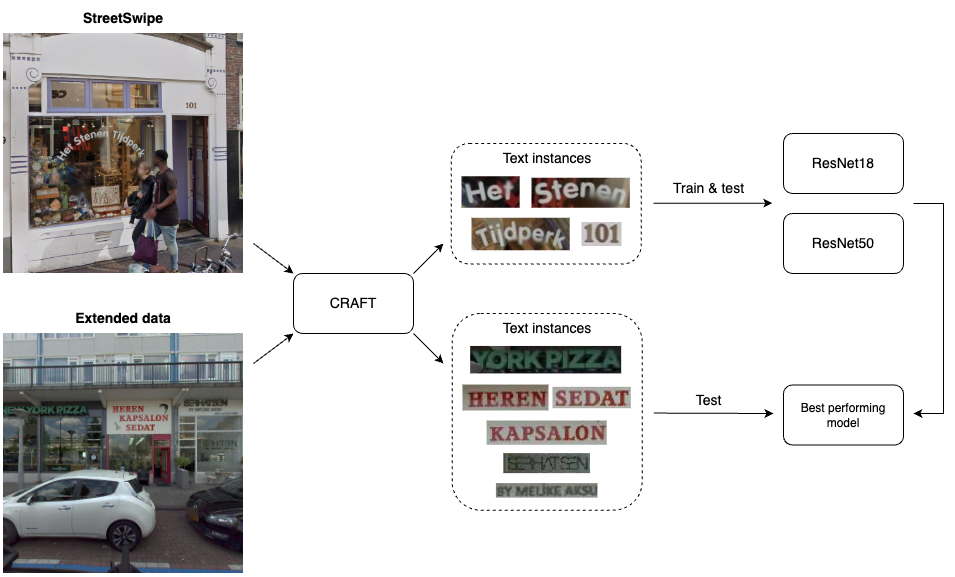
\includegraphics[width=\textwidth]{media/methodology/Pipeline2.png}
    \caption{Pipeline: Images of facades labelled gentrified or non-gentrified are first fed into the text detection model (CRAFT) to extract text instances. The ResNet50 is then trained and tested on instances from StreetSwipe. Subsequently, the model is tested on instances from the extended data.}
    \label{fig:pipeline}
\end{figure*}


\subsubsection{Scene-text detection - CRAFT}

The first task is to detect and extract signage in the images of both datasets, using the pre-trained CRAFT model via the EasyOCR Python package.

More specifically, the \textit{detect} method was used, with text confidence threshold \textit{(text\_threshold)} set to 0.75, bounding box extension \textit{(add\_margin)} set to 0, and all other parameters set to their default values.

Text instances are cropped out by their bounding boxes and grouped per image, per class. 


\subsubsection{Classification - ResNet}

In order to train and optimize the ResNets on StreetSwipe text instances, the data was split into training, validation and test sets with 80:10:10 ratio. The data was randomly shuffled prior to splitting to maintain class distribution per split. Table \ref{tab:data_split} shows the size of each split in the data.

\begin{table}[]
    \begin{tabular}{lrrrl}
    \cline{1-4}
            & \multicolumn{1}{r}{Total} &\multicolumn{1}{r}{Gentrified} & \multicolumn{1}{r}{Non-gentrified} &  \\ \cline{1-4}
Train       & 8063                      & 2092 (25.95\%)                & 5971 (74.05\%)           &  \\
Val         & 1008                      & 238 (23.61\%)                 & 770 (76.39\%)            &  \\
Test        & 1008                      & 280 (27.78\%)                 & 728 (72.22\%)            & 
    \end{tabular}
    \caption{Sample size per data split, per class}
    \label{tab:data_split}
\end{table}

Transformations applied to the training set include a random resized crop of size 224x224, random horizontal flip, transforming to tensor, and normalization with mean=[0.485, 0.456, 0.406] and std=[0.229, 0.224, 0.225]. For the validation and test sets, transformations include resizing to 224x224, a center crop, transforming to tensor, and normalization with mean and std as above.

Model training was done in PyTorch. Both the ResNet18 and ResNet50 were initialized with pre-trained ImageNet1K-V1 weights, with the final fully connected layer modified to give outputs of size 2. As a baseline, all the weights in the rest of the model were frozen and only the final layer was optimized; and no action was taken to account for class imbalance.

Next, the models were fine-tuned by optimizing all weights in the network. PyTorch's WeightedRandomSampling was applied to the training data loader to mitigate the effect of class imbalance, with each class' weight calculated as 1/(class size).

The loss function used was the cross entropy loss. The optimizer was stochastic gradient descent with a 0.9 momentum. StepLR learning rate decay scheduler was also implemented with a step size of 7 and gamma value of 0.1.

Manual hyperparameters tuning was done on the learning rate, batch size and number of training epochs. These choices of hyperparameters was motivated by the fact that throughout iterations of the models, there was no sign of overfitting, so hyperparameters such as dropout rate, L1 and L2 regularization were not considered.

\subsection{Evaluation}
Performance metrics - namely accuracy, precision, recall, and F1 score - were calculated for the classifier in validation and testing. The average metrics across classes (with macro averaging) were used to compare models per epoch, and additionally metrics per class were calculated. The metrics were implemented using torchmetrics' MulticlassAccuracy, MulticlassPrecision, MulticlassRecall, and MulticlassF1Score \cite{torchmetrics}. torchmetrics' ClasswiseWrapper was used to obtain metrics per class.

The formulas are as follow:
\[Accuracy = \frac{TP+TN}{TP+TN+FP+FN}\]
\[Precision = \frac{TP}{TP+FP}\]
\[Recall = \frac{TP}{TP+FN}\]
\[F1 Score = \frac{2 * Precision * Recall}{Precision + Recall}\]

% \section{Results}
\label{sec:results}

\subsection{Scene-text detection}
Some examples of the output text instances per class can be seen in Figure \ref{fig:instance_ex}.

{
\setlength\intextsep{7pt}
\begin{figure}[H]
\centering
\begin{subfigure}[b]{0.22\textwidth}
    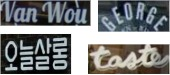
\includegraphics[width=\textwidth]{media/results/instances/instance_gen.jpg}
    \caption{Gentrified}
\end{subfigure}
\quad
\begin{subfigure}[b]{0.22\textwidth}
    
\includegraphics[width=\textwidth]{media/results/instances/instance_non.jpg}
    \caption{Non-gentrified}
\end{subfigure}
\caption{Text instances examples.}
\label{fig:instance_ex}
\end{figure}
}

Since there was no bounding box annotations of the signage, evaluation was done by visual inspection. It was found that the text detection model returned almost all text instances present in the original street view images, including non-horizontal and curved text. Cases where the model failed include very small, and therefore illegible texts, especially in lower resolution images. Additionally, the model also returned some noise, namely texts on street signs (e.g. traffic signs, street names), and watermarks ("©Google", as the images in StreetSwipe were originally from Google Street View) - these instances were manually removed.

\subsection{Classification}
\subsubsection{Baseline}
Test set results of the baseline model are shown in Table \ref{fig:baseline_metrics}. 

% {
% \setlength\intextsep{7pt}
\begin{table}[h]
\begin{tabular}{llcc}
\toprule
\multirow{2}{*}{Metrics}   & \multirow{2}{*}{Class} & \multicolumn{2}{c}{Baseline model}        \\ \cline{3-4} 
                           &                        & Classwise & Average                 \\ \hline
Accuracy                   & Gentrified             & 0.2143    & \multirow{2}{*}{0.5810} \\
                           & Non-gentrified         & 0.9478    &                         \\
Precision                  & Gentrified             & 0.6122    & \multirow{2}{*}{0.6852} \\
                           & Non-gentrified         & 0.7582    &                         \\
Recall                     & Gentrified             & 0.2143    & \multirow{2}{*}{0.5810} \\
                           & Non-gentrified         & 0.9478    &                         \\
F1-score                   & Gentrified             & 0.3175    & \multirow{2}{*}{0.5800} \\
                           & Non-gentrified         & 0.8425    &                         \\
\bottomrule
\end{tabular}
\vspace{\baselineskip}
\caption{Test set classwise and macro-averaged metrics of baseline model (ResNet50, no weighted sampling, no fine-tuning). This model achieved very high performance for non-gentrified signage, but performed poorly on gentrified signage, due to class imbalance.}
\label{fig:baseline_metrics}
\vspace{-8mm}
\end{table}
% }

\subsubsection{Fine-tuned}
The best performing model with ResNet18 architecture was found with learning rate set to 0.001, batch size 32, and 60 training epochs. The best performing model with ResNet50 architecture was found with learning rate set to 0.01, batch size 64, and 60 training epochs. The macro-averaged metrics across classes for these models are shown in Table \ref{fig:resnet_compare}. The fine-tuned ResNet50 had better performance, its classwise metrics are shown in Table \ref{fig:resnet50_cls}.

% {
% \setlength\intextsep{10pt}
\begin{table}[h!]
    \begin{tabular}{lcccc}
    \toprule
\multirow{2}{*}{Metrics} & \multicolumn{2}{c}{ResNet18} & \multicolumn{2}{c}{ResNet50} \\ \cmidrule(lr){2-3} \cmidrule(lr){4-5}
                         & Val           & Test          & Val           & Test         \\ \hline
Accuracy                 & 0.6497        & 0.6960        & 0.6506        & \textbf{0.7033}       \\
Precision                & 0.6185        & 0.6715        & 0.6209        & \textbf{0.6795}       \\
Recall                   & 0.6497        & 0.6960        & 0.6506        & \textbf{0.7033}       \\
F1-score                 & 0.6222        & 0.6781        & 0.6256        & \textbf{0.6865}       \\ \bottomrule
    \end{tabular}
    \vspace{\baselineskip}
    \caption{Macro-averaged metrics of the best-performing fine-tuned ResNet18 and ResNet50. Between these two models, the fine-tuned ResNet50 performed better.}
    \label{fig:resnet_compare}
    \vspace{-5mm}
\end{table}
% }

% {
% \setlength\intextsep{0pt}
\begin{table}[h!]
\begin{tabular}{llcc}
\toprule
\multirow{2}{*}{Metrics}   & \multirow{2}{*}{Class} & \multicolumn{2}{c}{ResNet50} \\ \cline{3-4} 
                           &                        & Val           & Test         \\ \hline
Accuracy                   & Gentrified             & 0.5714        & 0.6429       \\
                           & Non-gentrified         & 0.7299        & 0.7637       \\
Precision                  & Gentrified             & 0.3953        & 0.5114       \\
                           & Non-gentrified         & 0.8464        & 0.8476       \\
Recall                     & Gentrified             & 0.5714        & 0.6429       \\
                           & Non-gentrified         & 0.7299        & 0.7637       \\
F1-score                   & Gentrified             & 0.4674        & \textbf{0.5696}       \\
                           & Non-gentrified         & 0.7838        & \textbf{0.8035}       \\
\bottomrule
\end{tabular}
\vspace{\baselineskip}
\caption{Classwise metrics of best model (fine-tuned ResNet50). Even though there was clear improvements in classifying gentrified signage compared to the baseline model, this model still did better on non-gentrified signage - most notably shown in the F1-scores of each class.}
\label{fig:resnet50_cls}
\vspace{-7mm}
\end{table}
% }

\subsection{Testing on extended data}
The average and classwise metrics of the best model in classifying the extended data are presented in Table \ref{fig:resnet50_pano}.

% {
% \setlength\intextsep{2.65pt}
\begin{table}[h!]
\begin{tabular}{llcc}
\toprule
\multirow{2}{*}{Metrics}   & \multirow{2}{*}{Class} & \multicolumn{2}{c}{Extended data}   \\ \cline{3-4} 
                           &                        & Classwise & Average                 \\ \hline
Accuracy                   & Gentrified             & 0.5340    & \multirow{2}{*}{0.5807} \\
                           & Non-gentrified         & 0.6274    &                         \\
Precision                  & Gentrified             & 0.7359    & \multirow{2}{*}{0.5725} \\
                           & Non-gentrified         & 0.4092    &                         \\
Recall                     & Gentrified             & 0.5340    & \multirow{2}{*}{0.5807} \\
                           & Non-gentrified         & 0.6274    &                         \\
F1-score                   & Gentrified             & 0.6189    & \multirow{2}{*}{0.5571} \\
                           & Non-gentrified         & 0.4953    &                         \\
\bottomrule
\end{tabular}
\vspace{\baselineskip}
\caption{Macro-average and classwise metrics of the best model in classifying the extended data. Compared to the metrics on StreetSwipe's test set, there was a consistent decrease of approximately 10\% in all average metrics on this data. Notably, this decrease mainly came from a worsened performance in classifying non-gentrified signage.}
\label{fig:resnet50_pano}
\vspace{-5mm}
\end{table}
% }

\subsection{Inspecting model's output}

\subsubsection{Correct classifications}

StreetSwipe's signage per class with classification probability of 80\% and above were inspected. This showed the most typical and distinguishing characteristics of signage per class, which can be seen in Figure \ref{fig:output_vis}.

Gentrified signage were more similar in font types and often did not vary in text sizes, while non-gentrified signage used more types of fonts, sometimes more than one fonts on a single sign, and sometimes with varying text sizes and orientations. In addition, gentrified signs mostly had white texts, with minimal variation in background colors. Non-gentrified signs were the opposite: texts varied more in colors, as well as background colors; and the appearance of neon signage in this class was also notable. In terms of languages, gentrified signage had more English text, with very rare appearances of non-Latin languages (e.g. Korean), while non-gentrified ones were largely in Dutch, with appearances of some English, Chinese and Arabic. And finally, although out of scope of the study, the model also picked up graffiti as instances belonging to non-gentrified facades.


\subsubsection{Incorrect classifications} 

StreetSwipe's mis-classified signage per class with low (50-70\%) and high ($ \geq 80\% $) classification probabilities were inspected. The mis-classified instances with high certainty showed similar characteristics to correctly classified instances (gentrified signage: mainly white text, less variation in font styles and background colors; non-gentrified signage: more variation in fonts, text colors and background colors). On the other hand, mis-classified instances with lower certainty showed a more nuanced picture, whereby if distinguishing features per class appeared together in one signage (e.g. non-white text (more typical of non-gentrified) on white or dark background (more typical of gentrified), signal strength diminished and the model's outputs of the two classes were less obviously distinguishable. Results can be seen in Figure \ref{fig:output_vis_SS_incorrect}.


\subsubsection{Classifications on extended data}

Model's classifications on the extended data's signage with classification probability of 80\% and above were inspected (disregarding ground truth label). Signage classified per class followed the same characteristics learned from StreetSwipe. Results can be seen in Figure \ref{fig:output_vis_pano}.


\begin{figure*}[]
    \centering
    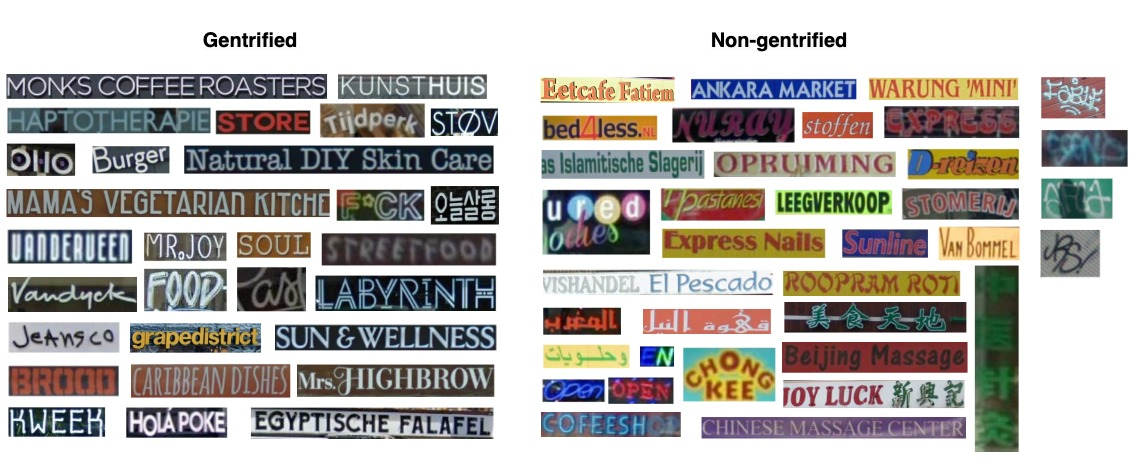
\includegraphics[width=0.8\textwidth]{media/results/output_vis-SS_correct1.jpg}
        \caption{StreetSwipe's correctly classified signage per class with probability of 80\% and above. Note how non-gentrified signage varied more in their characteristics (more font types, colors, and languages) while gentrified signage appeared more homogenized.}
        \label{fig:output_vis}
    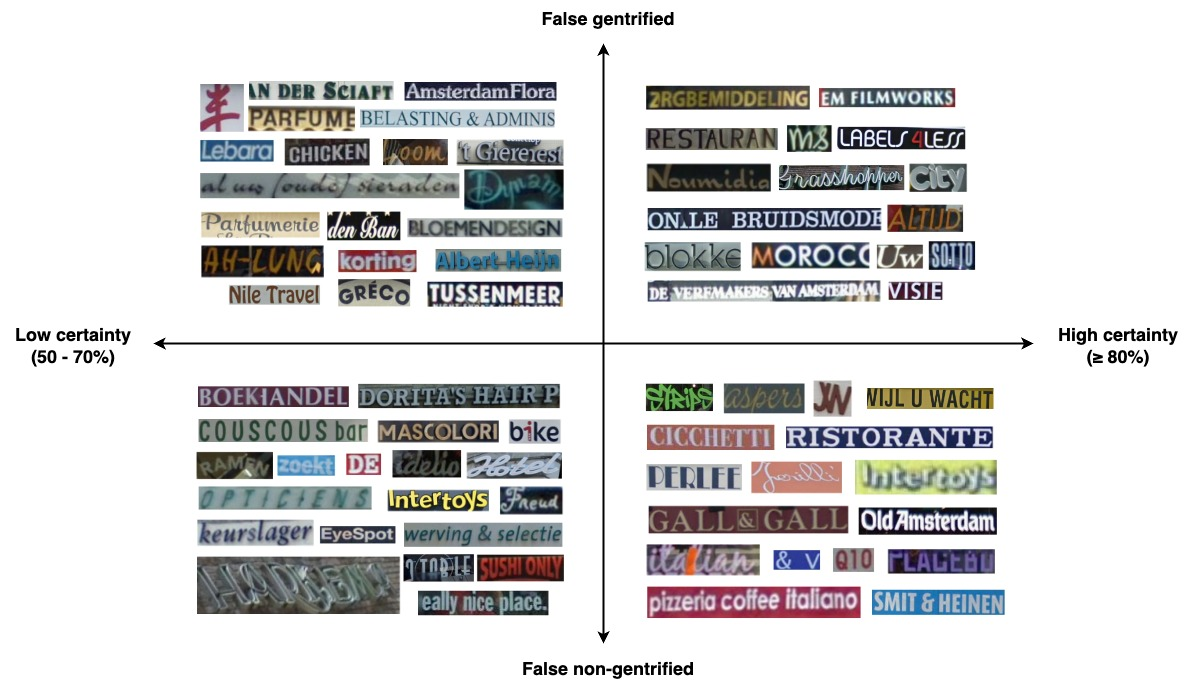
\includegraphics[width=0.9\textwidth]{media/results/output_vis-SS_incorrect.jpg}
        \caption{StreetSwipe's incorrectly classified signage per class, grouped by high and low classification certainty. Incorrect classifications with high certainty from both classes generally had the same characteristics as correctly classified instances. As classification certainty decreased, variations in fonts and colors were no longer distinctive across the two classes.}
        \label{fig:output_vis_SS_incorrect}
    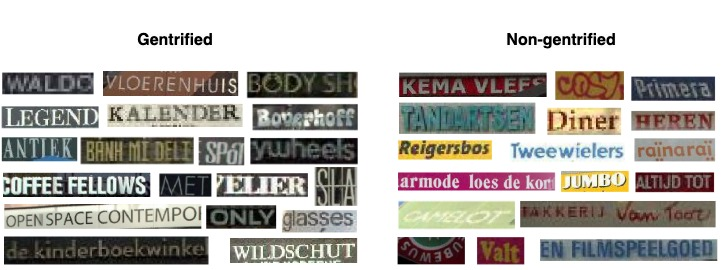
\includegraphics[width=0.6\textwidth]{media/results/output_vis-pano1.jpg}
        \caption{Model's classifications on the extended data's signage with classification probability of 80\% and above (disregarding ground truth label). It's notable how the model's inference on this data showed the same characteristics per class as in StreetSwipe.}
        \label{fig:output_vis_pano}
\end{figure*}
% % \newpage
\section{Discussion}
\label{sec:discussion}
% Compare your results with the state-of-the-art and reflect upon the results and limitations of the study. You can already hint at future work to which you come back in the conclusion section.
% Write your discussion here. Do not forget to use sub-sections. Normally, the discussion starts with comparing your results to other studies as precisely as possible. The limitations should be reflected upon in terms such as reproducibility,  scalability,  generalizability,  reliability  and  validity. It is also important to mention ethical concerns.


\subsection{Summarizing results}

In using a fine-tuned ResNet50, the current study was able to find the same patterns of gentrification in Amsterdam storefront signage characteristics as previous research, in terms of colors and fonts \cite{rahman_signage_2020, trinch_signsays_2017, snajdr_oldschool_2018, snajdr_preserve_2022}, as well as languages \cite{kasanga_map_2012, trinch_signsays_2017}

Using a image classification model had also enabled the study to make conclusions on fuzzy cases, via inspecting the model's mis-classified instances. These were instances where gentrified-labeled signs actually had the defining characteristics of non-gentrified signs, and thus were identified as such by the model with high certainty. Further, as classification certainty decreased, we were able to see signage with appearances untypical of any class. Variations in fonts and colors were no longer differentiating one class from another. Such output showed more nuances in identifying gentrification via signage. Signage alone could not always tell the full story, as signage of non-gentrified facades can still appear gentrified and vice versa, with strong and consistent visual signals found by the model. Especially for the cases of lower classification certainty, the model failed to tell apart gentrified from non-gentrified signs as signals from both classes appeared together. While we were able to see what signs looked like  beyond the most typical cases of (non-)gentrification (something previous studies did not point out), ultimately, these were the cases where the model failed to distinguish due to added nuances.

Utilizing street view imagery and computer vision had also enabled this study to overcome the limitations of past research in terms of generalizability. Past studies, in using labor-intensive manual data collection and qualitative methods, could only make conclusions on a neighborhood scale \cite{reades_understanding_2019, barton_exploration_2016}. Generalizability of the model was tested on a set of extended street view data, label as gentrified and non-gentrified based on census data. Two analyses were done on this set. Firstly, looking at the model's performance, there was a consistent decrease in performance of approximately 10\% in all average metrics. This suggests that given a gentrified neighborhood, not all signage in the neighborhood would be visually perceived as gentrified. Secondly, looking at the model's inference on this data, the same visual patterns were found for both classes. This supports the model's ability to identify visually (non-)gentrified signs from unseen data on a city-wide scale.

\subsection{Limitations}
\subsubsection{Data-related limitations}

StreetSwipe had the following limitations: 
\begin{itemize}
    \item The number of votes in pre-july 2020 version of the data was less than in the newer version. This could have lead to lower validity of the results.
    \item There was strong class imbalance, with 75\% of the data belonging to non-gentrified instances. This affected the model's performance in detecting gentrified instances.
    \item The data had varying dates, with some images dating back to 2009. While we technically could still learn perception, as the images were human-annotated in recent years, the results - especially conclusions made about visual characteristics of signage - should not be interpreted as fully representing the most up-to-date state of gentrification in Amsterdam.
\end{itemize}

The extended dataset had a limitation in terms of resolution: Text instances generally had much lower resolutions compared to StreetSwipe, and this is because the street view images were taken from a further distance. This could have contributed to model's lower performance on this set.

\subsubsection{Methodology-related limitations}
The methodology had the following limitations:

\begin{itemize}
    \item Cropping out text instances meant losing information on the entirety of the signage, such as where the text are placed (windows or above the stores' entrances, or standees, posters etc.), text density on signage, text size, total numbers of font types and colors used, which signage type and whether a combination of types (above entrance, on window, standee, neon, backlit) was used. These elements could have served as extra signals for better classification of signage.
    
    \item Cropping out text instances also led to lower reliability for semantic learning, as the majority of instances were single words or fragmented. Learning semantic meanings of text could have helped distinguishing between the classes, especially when instances have visual characteristics of the opposite class.
    
\end{itemize}

\subsection{Future research}
Some avenues for future studies are listed below:
\begin{itemize}
    \item Via object recognition, future studies can include more visual signals by identifying signage in their entirety, and not as (potentially fragmented) text instances. Then, text placement, text density, signage types etc. could be used as features. Further, this would also enable more reliability for semantic learning.

    \item Other features could be combined to aid model accuracy. Other visual indicators include the appearance of the rest of the buildings, what else appeared in the store facade other than signage (e.g. window displays, outdoor seating). Non-visual indicators include types of business, locations, neighborhood socio-economic indicators such as housing prices, residents' age, education level, income, etc. Similar to semantics, these features can further improve classification, especially when signage visual signals are a misdirection for the model.
    
    \item The mismatch in model performance on StreetSwipe and the extended data - or between visual and socio-economic gentrification - points to questions about the neighborhood's demographic makeup. It could be the case that displacement did not happen to old residents, or it did happen but business owners were able to cater to new residents and remained in the gentrified neighborhoods. A research in this direction calls for combining socio-demographic data in combination with street view imagery. A step further would be to incorporate time series data to enable an analysis into the process of neighborhood change, e.g. whether displacement took place over time.
\end{itemize}

% % \section{Conclusion}
% \label{sec:conclusion}
% % Answer each research question and address how the limitations of the study qualify the conclusion.
% Write your conclusion here. Be sure that the relation between the research gap and your contribution is clear. Be honest about how limitations in the study qualify the answer on the research question.

\bibliographystyle{ACM-Reference-Format}
\bibliography{bibliographies/references}

% \newpage
% % You can choose whether you prefer a single or double column appendix.
% Whatever you choose, you will need to stick to it throughout the appendix.
% For double column style, comment the next line.
\onecolumn

\appendix
\begin{appendices}

\section{Text instance sizes and aspect ratios}
\label{sec:apx:first_appendix}

% \subsection{Appendix 1.1: StreetSwipe text instance size and aspect ratio}
\begin{figure}[H]
    \centering
    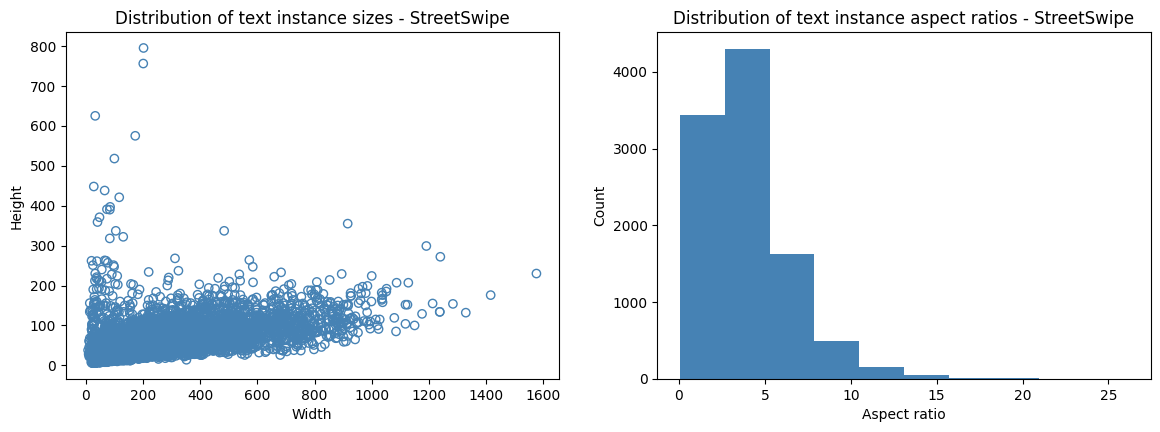
\includegraphics[width=\textwidth]{media/methodology/SS_ins_sz.png}
    \caption{StreetSwipe text instance size and aspect ratio}
    \label{fig:SS_ins_sz}
\end{figure}

% \subsection{Appendix 1.2: Extended data text instance size and aspect ratio}
\begin{figure}[H]
    \centering
    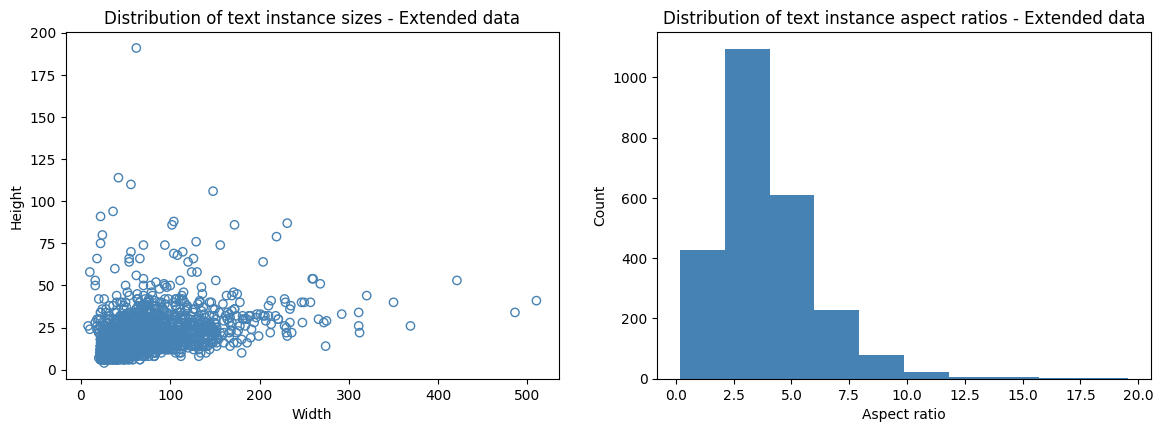
\includegraphics[width=\textwidth]{media/methodology/pano_ins_sz.png}
    \caption{Extended data text instance size and aspect ratio}
    \label{fig:pano_ins_sz}
\end{figure}

\end{appendices}


\end{document}

%%%%%%%%%%%%%%%%%%%%%%%%%%%%%%%%%%%%%%%%%%%%%%%%%%%%%%%%%%%%%%%%%%%%%%%%%%%%%%%%
%%%%%%%%%%%%%%%%%%%%%%%%%%%%%%%%%%%%%%%%%%%%%%%%%%%%%%%%%%%%%%%%%%%%%%%%%%%%%%%%